\documentclass{beamer}
% \documentclass[handout]{beamer}

% Paquetes
% ---------------------------------------------------------------------------- %
\usepackage[utf8]{inputenc}
\usepackage[spanish]{babel}
%\usepackage{listings}
%\usepackage{graphicx}
%\usepackage{xspace}
%\usepackage{enumitem}
%\usepackage{tikz}
%\usepackage{fancyvrb}
\usepackage{caption}
\usepackage{array}

% Configuración del 'theme'
% ---------------------------------------------------------------------------- %
\usetheme{Madrid}

\graphicspath{ {images/} }

% Definición de comandos
% ---------------------------------------------------------------------------- %
\newcommand{\code}[1]{\texttt{#1}\xspace}
\newcommand{\command}[1]{\texttt{\textcolor{greencmd}{#1}}}

\let\oldemph\emph
\renewcommand{\emph}[1]{\structure{#1}}

% Configuración de 'Title Page'
% ---------------------------------------------------------------------------- %
\title[Contenedores]{\textit{Contenedores}}
%\author{}
\institute[Sistemas Operativos]{Sistemas Operativos\\DC - FCEN - UBA}
\date[1C 2025]{23 de junio de 2025}

% Mostrar temario al cambiar de sección
% ---------------------------------------------------------------------------- %
\AtBeginSection[]
{
   \begin{frame}
        \frametitle{Menú para hoy}
        \tableofcontents[currentsection,currentsubsection]
   \end{frame}
}

% Diapositivas
% ---------------------------------------------------------------------------- %
\begin{document}

% ---------------------------------------------------------------------------- %
\begin{frame}[plain,t]
\titlepage
\end{frame}

% ---------------------------------------------------------------------------- %
%The next statement creates the title page.
\begin{frame}
\frametitle{Menú para hoy}
\tableofcontents
\end{frame}
%------------------------------------------------------------
\section{Virtualización}
% ---------------------------------------------------------------------------- %
    \begin{frame}
    \frametitle{Virtualización}
    \framesubtitle{Definición}
        \begin{itemize}
            \item Definición: \pause es la posibilidad de que un conjunto de recursos físicos se vean como varias copias de recursos lógicos.\pause
            \item Objetivos: \pause
            \begin{itemize}
                \item Portabilidad.
                \item Aislamiento.
                \item Particionamiento de HW.
                \item Migración entre HW sin pérdida de servicio.
                \item Correr sistemas viejos.
                \item ...
            \end{itemize}
        \end{itemize}
    \end{frame}
% ---------------------------------------------------------------------------- %
    \begin{frame}
    \frametitle{Virtualización}
    \framesubtitle{Tipos de virtualización}
        \begin{itemize}
            \item Tipos de virtualización:
            \begin{itemize}
                \item Simulación \pause
                \begin{figure}
                    \captionsetup{
                        justification=centering,
                        font=scriptsize,
                        width=0.8\textwidth
                    }
                    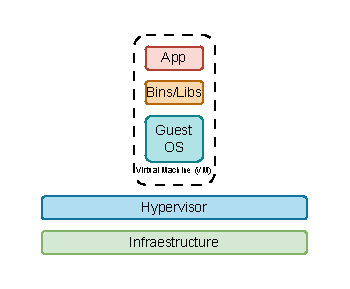
\includegraphics[width=0.6\textwidth]{images/virtualization_com_0.pdf}
                \end{figure}
            \end{itemize}
        \end{itemize}
    \end{frame}
% ---------------------------------------------------------------------------- %
    \begin{frame}
    \frametitle{Virtualización}
    \framesubtitle{Tipos de virtualización}
        \begin{itemize}
            \item Tipos de virtualización:
            \begin{itemize}
                \item Simulación
                \begin{figure}
                    \captionsetup{
                        justification=centering,
                        font=scriptsize,
                        width=0.8\textwidth
                    }
                    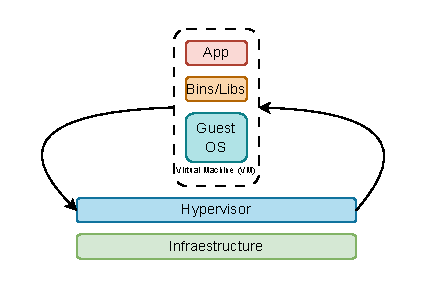
\includegraphics[width=0.6\textwidth]{images/simulation_com_1.pdf}
                \end{figure}
            \end{itemize}
        \end{itemize}
    \end{frame}
% ---------------------------------------------------------------------------- %
    \begin{frame}
    \frametitle{Virtualización}
    \framesubtitle{Tipos de virtualización}
        \begin{itemize}
            \item Tipos de virtualización:
            \begin{itemize}
                \item Simulación
                \item Emulación  \pause
                \begin{figure}
                    \captionsetup{
                        justification=centering,
                        font=scriptsize,
                        width=0.8\textwidth
                    }
                    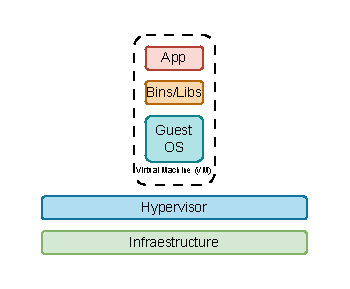
\includegraphics[width=0.6\textwidth]{images/virtualization_com_0.pdf}
                \end{figure}
            \end{itemize}
        \end{itemize}
    \end{frame}
% ---------------------------------------------------------------------------- %
    \begin{frame}
    \frametitle{Virtualización}
    \framesubtitle{Tipos de virtualización}
        \begin{itemize}
            \item Tipos de virtualización:
            \begin{itemize}
                \item Simulación
                \item Emulación
                \begin{figure}
                    \captionsetup{
                        justification=centering,
                        font=scriptsize,
                        width=0.8\textwidth
                    }
                    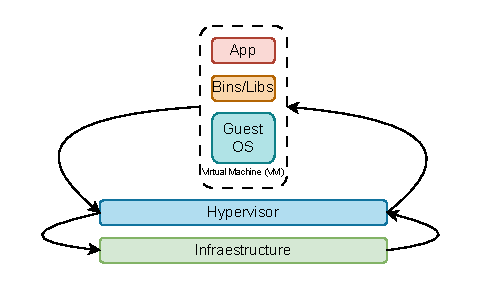
\includegraphics[width=0.6\textwidth]{images/emulation_com_1.pdf}
                \end{figure}
            \end{itemize}
        \end{itemize}
    \end{frame}
% ---------------------------------------------------------------------------- %
    \begin{frame}
    \frametitle{Virtualización}
    \framesubtitle{Tipos de virtualización}
        \begin{itemize}
            \item Tipos de virtualización:
            \begin{itemize}
                \item Simulación
                \item Emulación
                \item Asistida por HW \pause
                \begin{figure}
                    \captionsetup{
                        justification=centering,
                        font=scriptsize,
                        width=0.8\textwidth
                    }
                    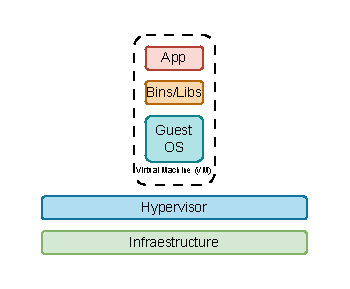
\includegraphics[width=0.6\textwidth]{images/virtualization_com_0.pdf}
                \end{figure}
            \end{itemize}
        \end{itemize}
    \end{frame}
% ---------------------------------------------------------------------------- %
    \begin{frame}
    \frametitle{Virtualización}
    \framesubtitle{Tipos de virtualización}
        \begin{itemize}
            \item Tipos de virtualización:
            \begin{itemize}
                \item Simulación
                \item Emulación
                \item Asistida por HW
                \begin{figure}
                    \captionsetup{
                        justification=centering,
                        font=scriptsize,
                        width=0.8\textwidth
                    }
                    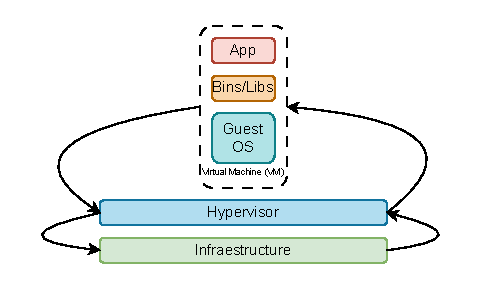
\includegraphics[width=0.6\textwidth]{images/hw-assisted_com_1.pdf}
                \end{figure}
            \end{itemize}
        \end{itemize}
    \end{frame}
% ---------------------------------------------------------------------------- %
    \begin{frame}
    \frametitle{Virtualización}
    \framesubtitle{Hypervisor vs SO + Hypervisor}
        \begin{figure}
            \captionsetup{
                justification=centering,
                font=scriptsize,
                width=0.8\textwidth
            }
            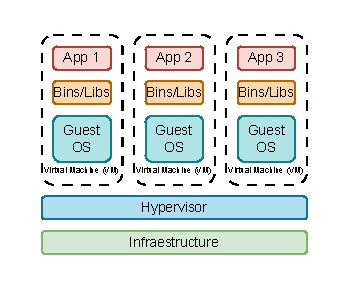
\includegraphics[width=0.6\textwidth]{images/virtualization_hyper_hosted.pdf}
        \end{figure}
    \end{frame}
% ---------------------------------------------------------------------------- %
    \begin{frame}
    \frametitle{Virtualización}
    \framesubtitle{Hypervisor vs SO + Hypervisor}
        \begin{figure}
            \captionsetup{
                justification=centering,
                font=scriptsize,
                width=0.8\textwidth
            }
            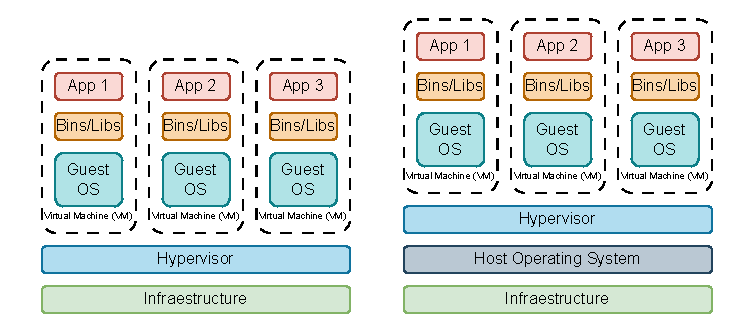
\includegraphics[width=\textwidth]{images/virtualization_so_hosted.pdf}
        \end{figure}
    \end{frame}
% ---------------------------------------------------------------------------- %
\section{Contenedores}
% ---------------------------------------------------------------------------- %
    \begin{frame}
        \frametitle{Contenedores}
        \framesubtitle{Definición}
    
        \begin{itemize}
            \item ¿Es un tipo de virtualización? \pause No, no son una virtualización completa. \pause
            \item ¿Cómo funciona? \pause Se apoya en funciones del kernel de linux (como Namespaces, Cgroups y OverlayFS). \pause
        \end{itemize}
    
        \begin{figure}
            \captionsetup{
                justification=centering,
                font=scriptsize,
                width=0.8\textwidth
            }
            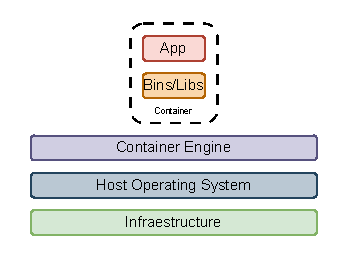
\includegraphics[width=0.6\textwidth]{images/container_com_0.pdf}
        \end{figure}
    \end{frame}
% ---------------------------------------------------------------------------- %
    \begin{frame}
        \frametitle{Contenedores}
        \framesubtitle{Definición}
    
        \begin{itemize}
            \item ¿Es un tipo de virtualización? No, no son una virtualización completa
            \item ¿Cómo funciona? Se apoya en funciones del kernel de linux (como Namespaces, Cgroups y OverlayFS)
        \end{itemize}
    
        \begin{figure}
            \captionsetup{
                justification=centering,
                font=scriptsize,
                width=0.8\textwidth
            }
            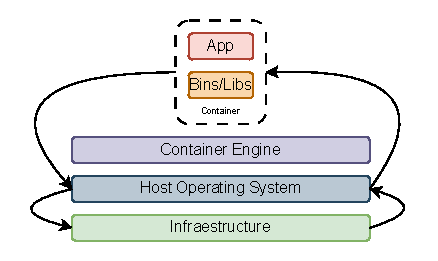
\includegraphics[width=0.6\textwidth]{images/container_com_1.pdf}
        \end{figure}
    \end{frame}
% ---------------------------------------------------------------------------- %
    \begin{frame}
        \frametitle{Contenedores}
        \framesubtitle{Definición}
        
        \begin{figure}
            \captionsetup{
                justification=centering,
                font=scriptsize,
                width=0.8\textwidth
            }
            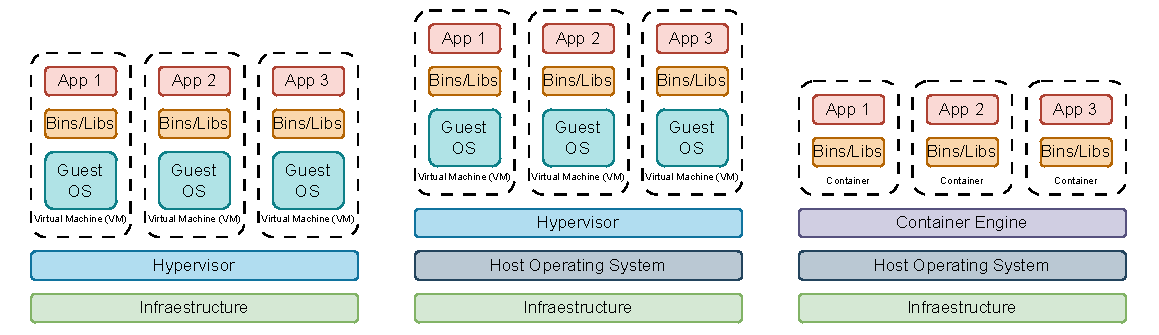
\includegraphics[width=\textwidth]{images/container_so_hosted.pdf}
        \end{figure}
    \end{frame}
% ---------------------------------------------------------------------------- %
\section{Imágenes}
% ---------------------------------------------------------------------------- %
    \begin{frame}
        \frametitle{Imágenes}
        \framesubtitle{Definición}
    
        \begin{itemize}
            \item Imágen de VM (VM Image): \pause Es un archivo que contiene un disco virtual que tiene instalado un sistema operativo, que el hipervisor la arranca como si fuese un servidor físico. \pause
            \item Imagen de container (Container Image): \pause Es es un archivo que incluye todos los archivos, binarios, bibliotecas y configuraciones, para poder ejecutar un contenedor a través de un container engine. \pause
        \end{itemize}
    
        \begin{figure}
            \captionsetup{
                justification=centering,
                font=scriptsize,
                width=0.8\textwidth
            }
            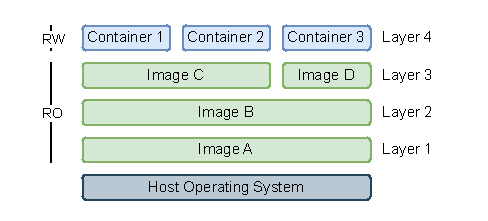
\includegraphics[width=0.6\textwidth]{images/OverlayFS.pdf}
        \end{figure}
    \end{frame}
% ---------------------------------------------------------------------------- %
    \begin{frame}
    \frametitle{Dockerfile}
    \framesubtitle{Comandos}
        \begin{block}{}
        \begin{itemize}
            \item FROM: Crear una nueva etapa de compilación a partir de una imagen base.
            \item WORKDIR: Cambiar directorio de trabajo.
            \item RUN: Ejecutar comandos de compilación.
            \item COPY: Copiar archivos y directorios.
            \item EXPOSE: Describe en qué puertos está escuchando tu aplicación.
            \item CMD: Especificar comandos predeterminados.
            \item ...
        \end{itemize}
        \end{block}
        \footnotetext{\textbf{https://docs.docker.com/reference/dockerfile/}}   
    \end{frame}
% ---------------------------------------------------------------------------- %
    \begin{frame}
    \frametitle{Docker Image}
    \framesubtitle{Construcción de una imagen}
        \begin{block}{}
        \begin{itemize}
            \item docker build -t \<image\_name\> \textit{\# Construye una Imagen a partir de un  Dockerfile}
            \item docker rmi \<image\_name\> \textit{\# Borra la imagen}
            \item ...
        \end{itemize}
        \end{block}

        \pause
        ¿Y donde quedan guardados estos archivos (imágenes)?
        
        \footnotetext{\textbf{https://docs.docker.com/reference/cli/docker/}}   
    \end{frame}
% ---------------------------------------------------------------------------- %
\begin{frame}
    \frametitle{Docker Image}
    \framesubtitle{¿Como funciona por debajo?}
    \begin{itemize}
        \item En el fondo Docker usa \emph{OverlayFS}, un \emph{unionFS}.
        \item Un unionFS permite agarrar diferentes file systems y crear un union de sus contenidos.
        \item Donde la capa mas alta provee una vision de todas las capas inferiores
        \item Si archivos duplicados se encuentran, la capa superior tiene privilegio sobre la capa inferior.
        \item Es decir, los archivos que se encuentran en ambas capas, solo se va a mostrar los que esten en la capa superior, en la capa de union.
    \end{itemize}
    \begin{flushleft}
    \begin{figure}
            \captionsetup{
                justification=raggedright,
                font=scriptsize,
                width=0.8\textwidth
            }
            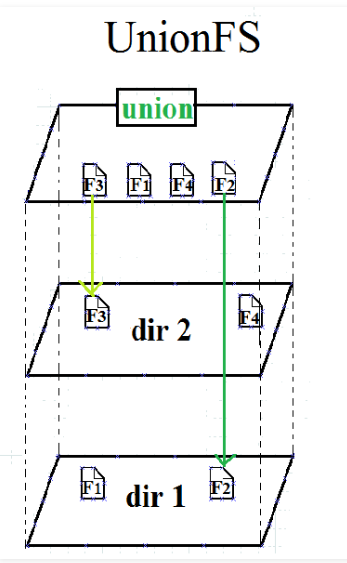
\includegraphics[width=0.15\textwidth]{images/unionfs5.png}
        \end{figure}
    \end{flushleft}
    \end{frame}
% ---------------------------------------------------------------------------- %
\begin{frame}
    \frametitle{Docker Image}
    \framesubtitle{¿Como funciona por debajo?}
    \begin{itemize}
        \item Docker a sus capas inferiores le dice \emph{Physical layers} y la capa de union \emph{Logical o overlay Layer}.
        \item Cada entrada dentro de un Dockerfile es una \emph{Physical layers} que se va apilando una arriba de la otra
        \item Cuando tenemos el contenedor corriendo, ahi estamos en la capa mas alta
    \end{itemize}
    \begin{flushleft}
    \begin{figure}
            \captionsetup{
                justification=raggedright,
                font=scriptsize,
                width=0.8\textwidth
            }
            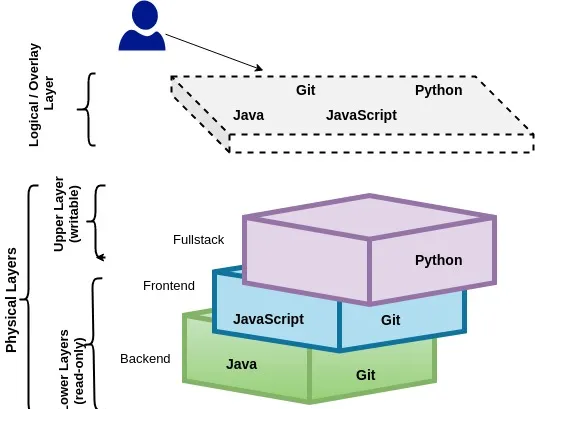
\includegraphics[width=0.4\textwidth]{images/dockerfs.png}
        \end{figure}
    \end{flushleft}
    \end{frame}
% ---------------------------------------------------------------------------- %
    \begin{frame}
    \frametitle{Registry}
    \framesubtitle{Almacenamiento de imágenes}
        \begin{block}{}
        \begin{itemize}
            \item Local \\
            docker images \textit{\# Lista imágenes locales.} \\
            ...
        \end{itemize}
        \end{block}

        \pause

        \begin{block}{}
        \begin{itemize}
            \item Registry \\
            docker login -u \<username\> \textit{\# Login a Docker Hub.} \\
            docker push \<username\>/\<image\_name\> \textit{\# Publica una imagen en Docker Hub.} \\
            docker search \<image\_name\> \textit{\# Busca una imagen en Docker Hub} \\
            docker pull \<image\_name\> \textit{\# Trae una imagen desde Docker Hub} \\
            ...
        \end{itemize}
        \end{block}
        
        \footnotetext{\textbf{https://hub.docker.com/search}}   
    \end{frame}
% ---------------------------------------------------------------------------- %
\section{Motor de contenedores}
% ---------------------------------------------------------------------------- %
    \begin{frame}
    \frametitle{Motor de contenedores}
    \framesubtitle{Almacenamiento de imágenes}

        \begin{block}{}
        \begin{itemize}
            \item docker run \<image\_name\> \textit{\# Crea y ejecuta un contenedor a partir de una imagen.}
            \item docker start|stop \<container\_name\> \textit{\# Inicia o para un container.}
            \item docker rm \<container\_name\> \textit{\# Remueve el contenedor.}
            \item docker ps \textit{\# Lista los contenedores que están ejecutando.}
            \item docker container stats \textit{\# Muestra el estado del uso de los recursos.}
            \item docker exec \<container\_name\> \<command\> \textit{\# Ejecuta el comando dentro del contenedor.}
            \item docker logs \<container\_name\> \textit{\# Muestra los logs del contenedor.}
        \end{itemize}
        \end{block}
        
        \footnotetext{\textbf{https://docs.docker.com/reference/cli/docker/}}   
    \end{frame}
% ---------------------------------------------------------------------------- %    
\section{Cierre}
% ---------------------------------------------------------------------------- %
    \begin{frame}
    \frametitle{Siguientes pasos}

    \begin{figure}
        \captionsetup{
            justification=centering,
            font=scriptsize,
            width=0.8\textwidth
        }
        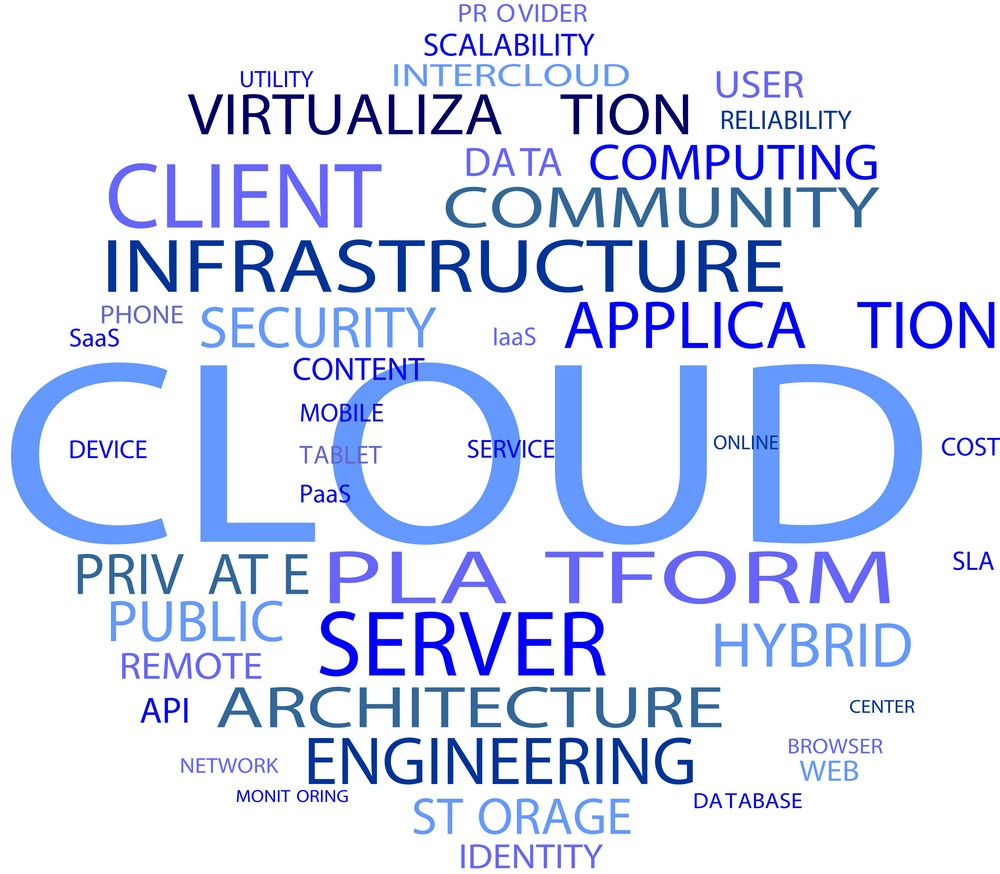
\includegraphics[width=0.6\textwidth]{images/cloud.jpg}
    \end{figure}
          
    \end{frame}
% ---------------------------------------------------------------------------- %
    \begin{frame}
    \frametitle{Siguientes pasos}

    \begin{figure}
        \captionsetup{
            justification=centering,
            font=scriptsize,
            width=0.8\textwidth
        }
        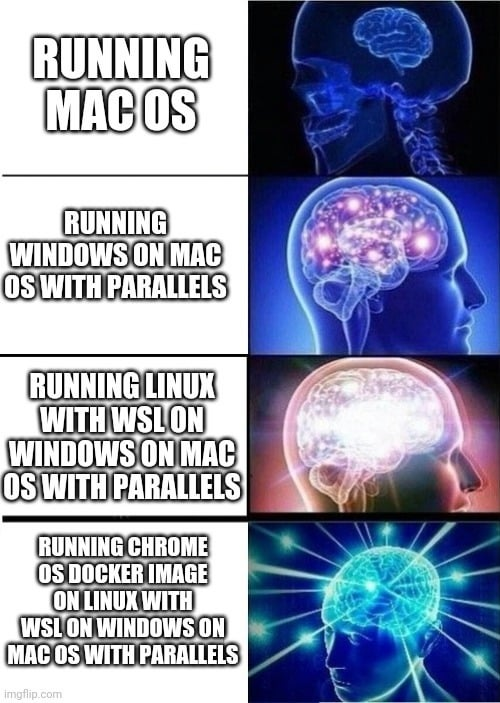
\includegraphics[width=0.45\textwidth]{images/end.jpg}
    \end{figure}
    \end{frame}
% ---------------------------------------------------------------------------- %

\end{document}
